\documentclass[12pt,letterpaper]{article}

\usepackage{amsmath, amsthm}
\usepackage{microtype, parskip}
\usepackage[comma,numbers,sort&compress]{natbib}
\usepackage{lineno}
\usepackage{docmute}
\usepackage{caption, subcaption, multirow, morefloats, rotating}
\usepackage{wrapfig}

\frenchspacing

\begin{document}

\section*{Results}

Posterior results take one of two forms: direct inspection of parameter estimates, and downstream estimates of diversity and diversification rates. For the former, both the pure-presence and birth-death models (Eq. \ref{eq:pure_presence}, and \ref{eq:birth_death} are inspected. For the latter, only posterior estimates from the birth-death model are considered; the reason for this is explained below in the comparison of the models' posterior predictive check results.

\subsection*{Comparing parameter estimates from the pure-presence and birth-death models}

% look at the posterior predictive checks
%   which model has better fit
%   what does that mean?

Comparison of the posterior predictive performance of the pure-presence and birth-death models reveals a striking difference in quality of the models' fits to the data (Fig. \ref{fig:ppc_pure_presence} and \ref{fig:ppc_birth_death}). The birth-death model is clearly able to reproduce the observed average number of occurrence, in contrast to the pure-birth model which greatly underestimates the ovserved average number of occurrences. The interpretation of these results is that the results of the birth-death model are more representative of the data than the pure-presence model, though further inspection of the posterior parameter estimates can provide further insight into why these models give different posterior predictive results \citep{Gelman2013d}.

\begin{figure}[ht]
  \centering
  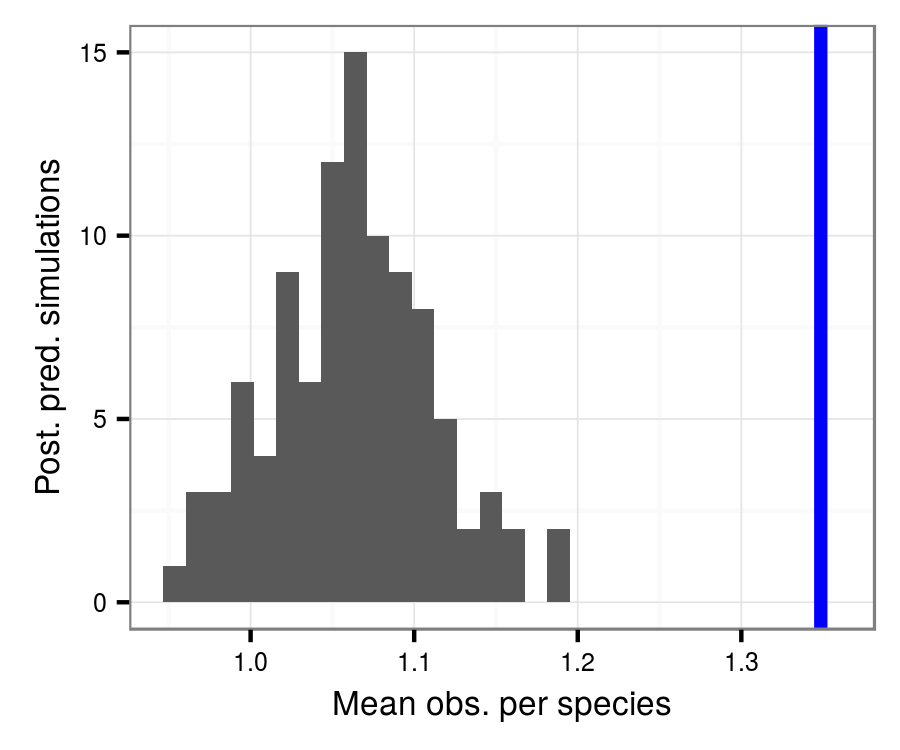
\includegraphics[width=\textwidth,height=0.4\textheight,keepaspectratio=true]{figure/pred_occ}
  \caption[Posterior predictive check for pure-presence model]{Comparison of the average observed number of occurrences per species (blue line) to the average number of occurrences from 100 posterior predictive datasets using the posterior estimates from the pure-presence model.}
  \label{fig:ppc_pure_presence}
\end{figure}

\begin{figure}[ht]
  \centering
  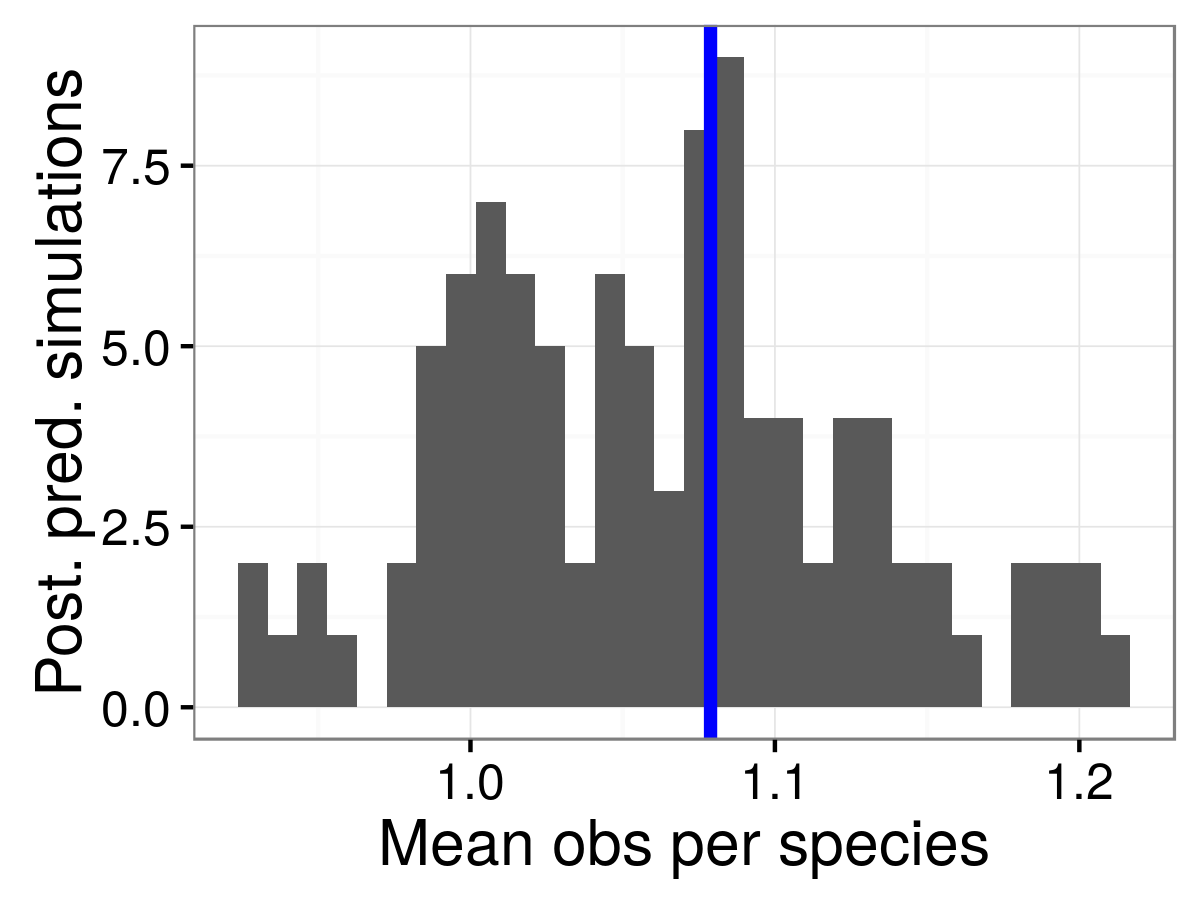
\includegraphics[width=\textwidth,height=0.4\textheight,keepaspectratio=true]{figure/pred_occ_bd}
  \caption[Posterior predictive check for birth-death model]{Comparison of the average observed number of occurrences per species (blue line) to the average number of occurrences from 100 posterior predictive datasets using the posterior estimate from the birth-death model.}
  \label{fig:ppc_birth_death}
\end{figure}


% need to inspect the posterior estimates in order to understand the differences
%   ecotype occurrence (pp), origination + survival (bd) probabilities
%   effect of mass on 
%     preservation (pp, bd)
%     occurrence (pp)
%     origination + survival (bd)
%   group-level covariates on 
%     occurrence (pp)
%     origination + survival (bd)

Occurrence probabilities estimated from the pure-presence model (Fig. \ref{fig:eco_occur}) are much more similar to the origination estimates from the birth-death model (Fig. \ref{fig:eco_origin}) than the estimates of survival probability (Fig. \ref{fig:eco_survival}). 

In general, both occurrence probabilities estimated from the pure-presence model (Fig. \ref{fig:eco_occur}) and origination probabilities estimated from the birth-death model (fig. \ref{fig:eco_origin}) increase with time. Notable, ecotypes with arboreal components do not follow this average; instead, occurrence and origination probabilities appear relatively flat for most of the Cenozoic.

The dramatic differences between origination and survival probabilities indicate how different these processes are, and may be responsible for the better posterior predictive perfomance of the birth-death model over the pure-presence model (Fig. \ref{fig:ppc_pure_presence}, and \ref{fig:ppc_birth_death}). While the estimates of both time series have high variance, what is striking is how mean origination probability changes over time while in general survival probabilities have relatively stable means (Fig. \ref{fig:eco_origin}, and \ref{fig:eco_survival}).

Estimates of origination probabilities appear to have less uncertainty than for survival (Fig. \ref{fig:eco_origin}, and \ref{fig:eco_survival}).


\begin{figure}[ht]
  \centering
  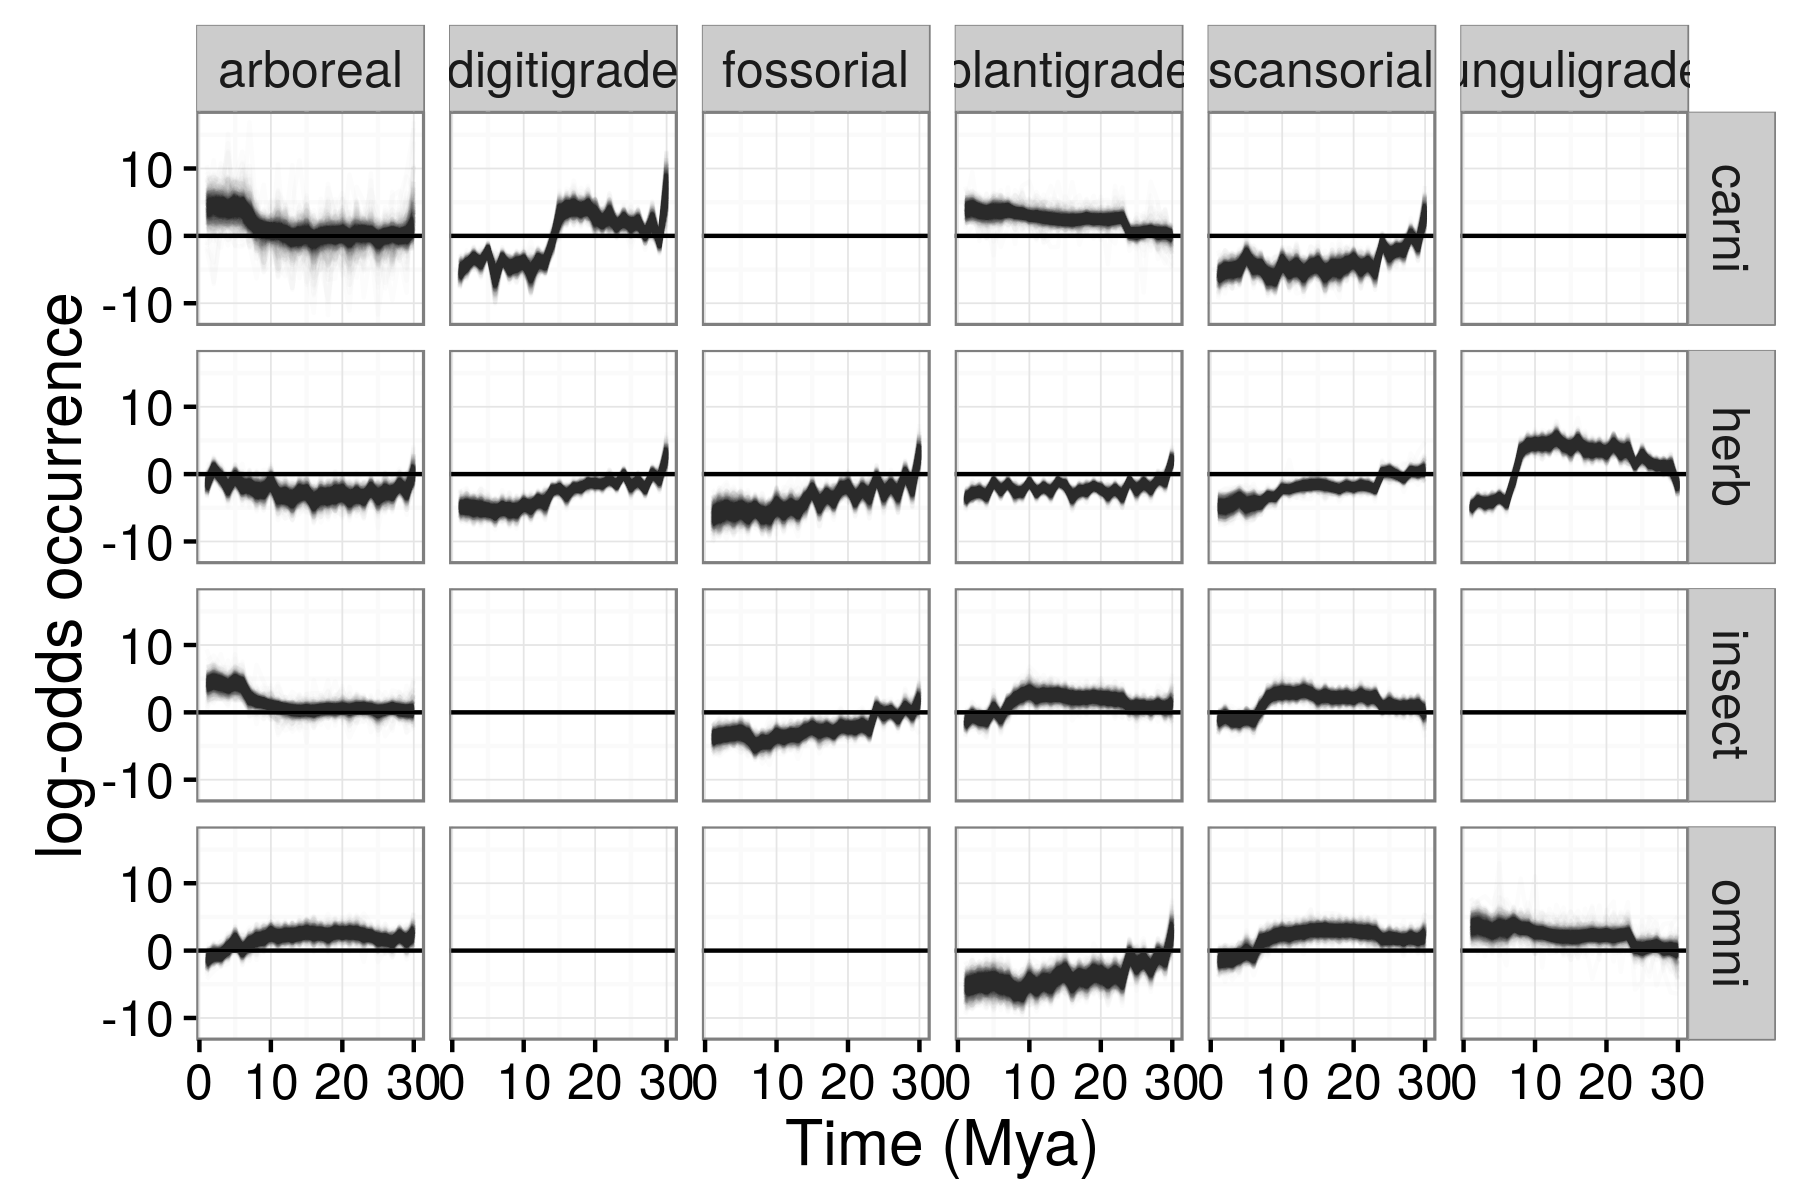
\includegraphics[width=\textwidth,height=0.8\textheight,keepaspectratio=true]{figure/ecotype_occurrence}
  \caption[Ecotype occurrence probability estimated from the pure-presence model]{Probability of a mammal ecotype occurring over time as estimated from the pure-presence model. Each panel depicts 100 random samples from the model's posterior. The columns are by locomotor category and rows by dietary category; their intersections are the observed and analyzed ecotypes. Panels with no lines are ecotypes not observed in the dataset.}
  \label{fig:eco_occur}
\end{figure}

\begin{figure}[ht]
  \centering
  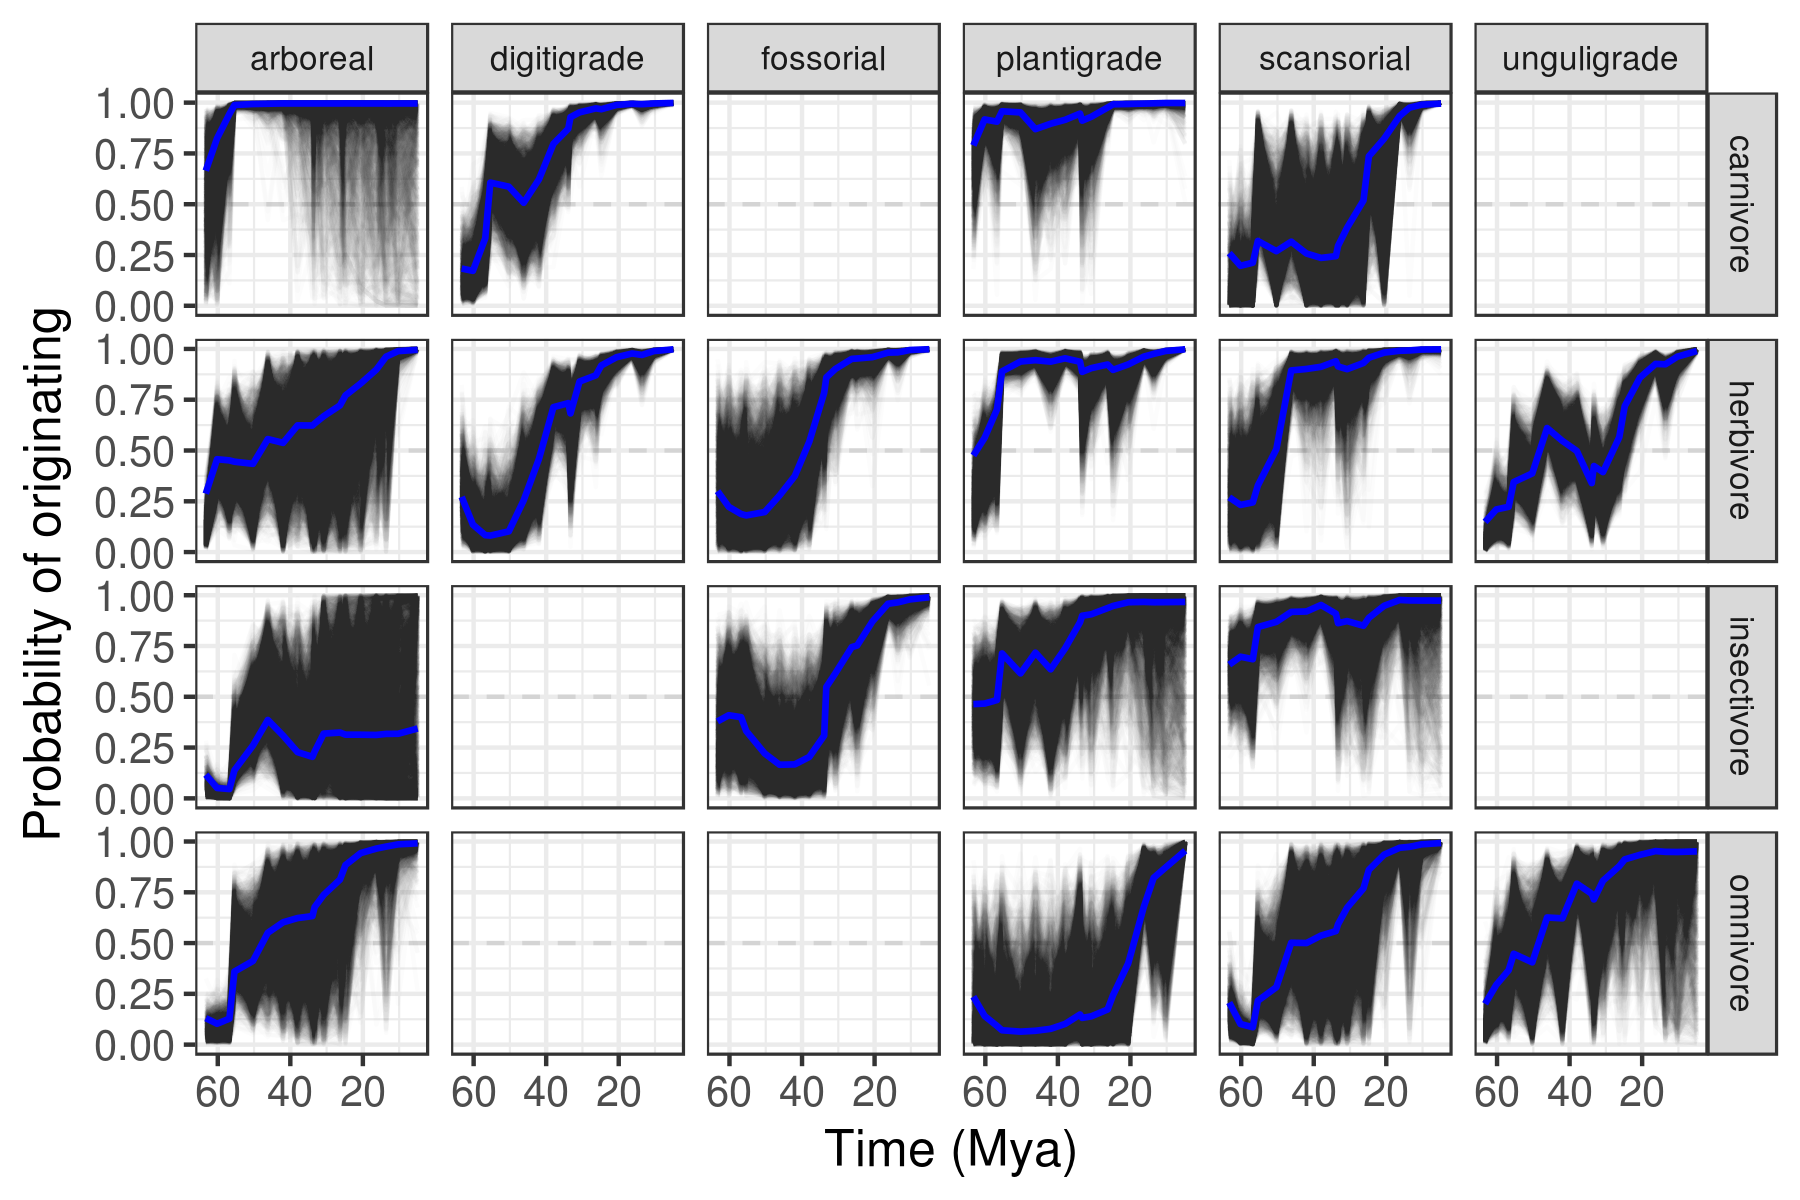
\includegraphics[width=\textwidth,height=0.8\textheight,keepaspectratio=true]{figure/ecotype_origin_bd}
  \caption[Ecotype origination probability estimated from the birth-death model]{Probability of a mammal ecotype origination probabliities at each time point as estimated from the birth-death model. Each panel depicts 100 random samples from the model's posterior. The columns are by locomotor category and rows by dietary category; their intersections are the observed and analyzed ecotypes. Panels with no lines are ecotypes not observed in the dataset.}
  \label{fig:eco_origin}
\end{figure}

\begin{figure}[ht]
  \centering
  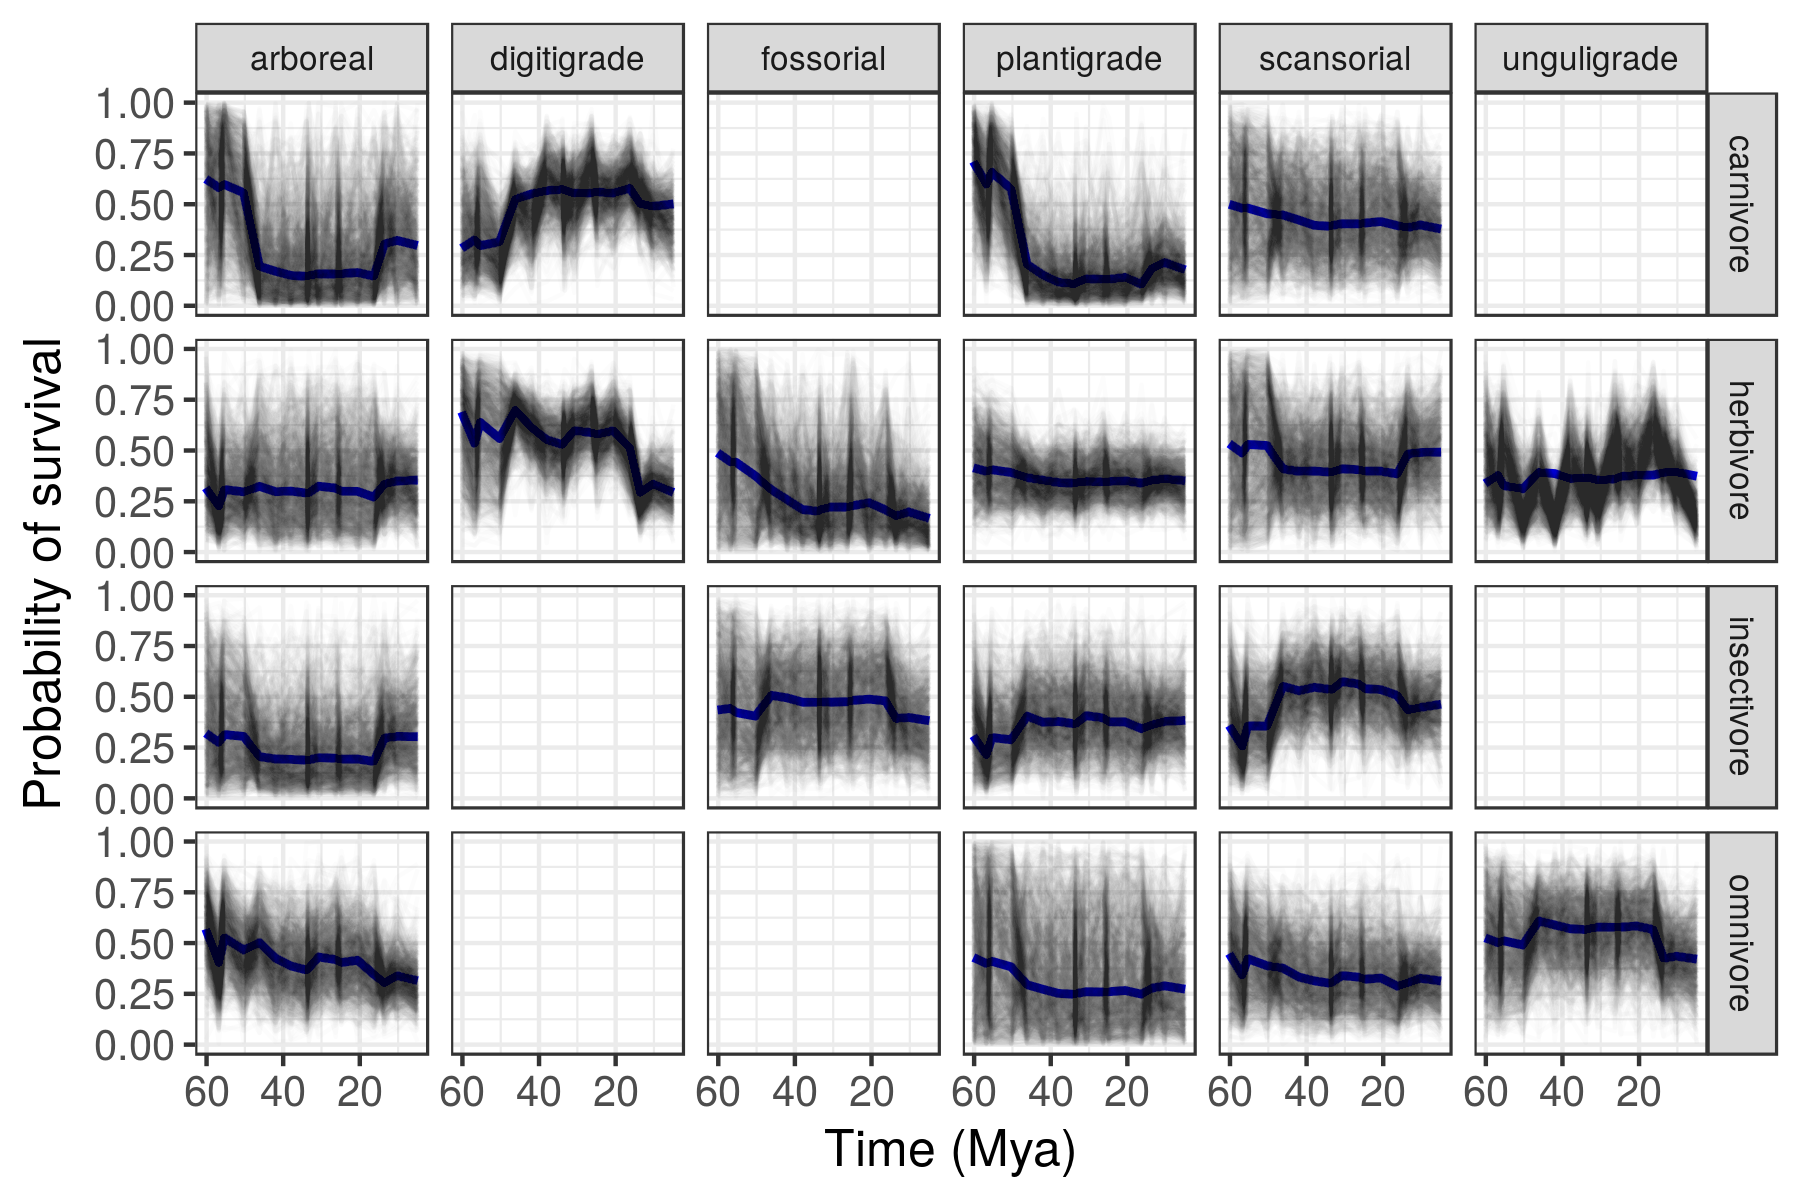
\includegraphics[width=\textwidth,height=0.8\textheight,keepaspectratio=true]{figure/ecotype_survival_bd}
  \caption[Ecotype survival probability estimated from the birth-death model]{Probability of a mammal ecotype survival probabilities at each time point as estimated from the birth-death model. Each panel depicts 100 random samples from the model's posterior. The columns are by locomotor category and rows by dietary category; their intersections are the observed and analyzed ecotypes. Panels with no lines are ecotypes not observed in the dataset.}
  \label{fig:eco_survival}
\end{figure}


For both the pure-presence and birth-death models there appears to be little effect of mass on the probability of observing a present species (Fig. \ref{fig:mass_preserve_pure_pres}, and \ref{fig:mass_preserve_bd}). These results may be unexpected given that it is generally assumed that larger mammals are more likely to have been collected than smaller mammals CITATION. However, collection is not preservation; 


\begin{figure}[ht]
  \centering
  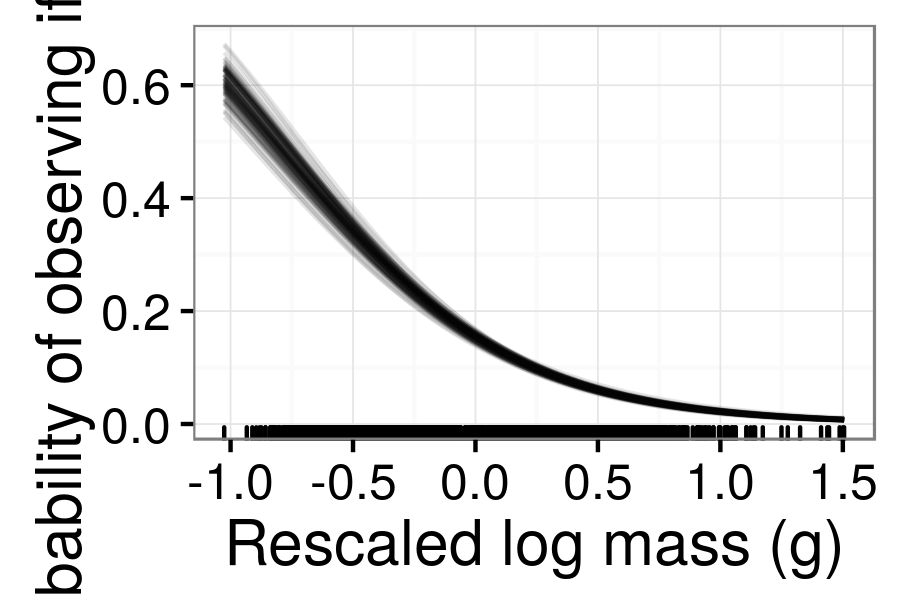
\includegraphics[width=\textwidth,height=0.8\textheight,keepaspectratio=true]{figure/mass_on_samp}
  \caption[Estimates of the effect of mass on observation probability from the pure-presence model]{Estimates of the effect of species mass on probability of observing a present species (\(p\)). Mass has been log-transformed, centered, and rescaled; this means that a mass of 0 corresponds to the mean of log-mass of all observed species and that mass is in standard deviation units. Estimates are from the pure-presence model.}
  \label{fig:mass_preserve_pure_pres}
\end{figure}

\begin{figure}[ht]
  \centering
  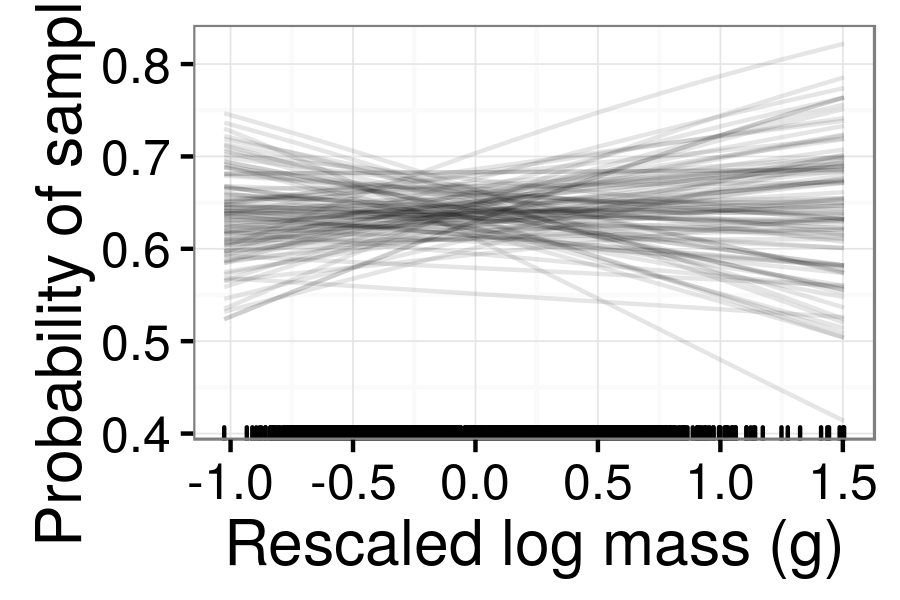
\includegraphics[width=\textwidth,height=0.8\textheight,keepaspectratio=true]{figure/mass_on_samp_bd}
  \caption[Estimates of the effect of mass on observation probability from the birth-death model]{Estimates of the effect of species mass on probability of observing a present species (\(p\)). Mass has been log-transformed, centered, and rescaled; this means that a mass of 0 corresponds to the mean of log-mass of all observed species and that mass is in standard deviation units. Estimates are from the birth-death model.}
  \label{fig:mass_preserve_bd}
\end{figure}

\begin{figure}[ht]
  \centering
  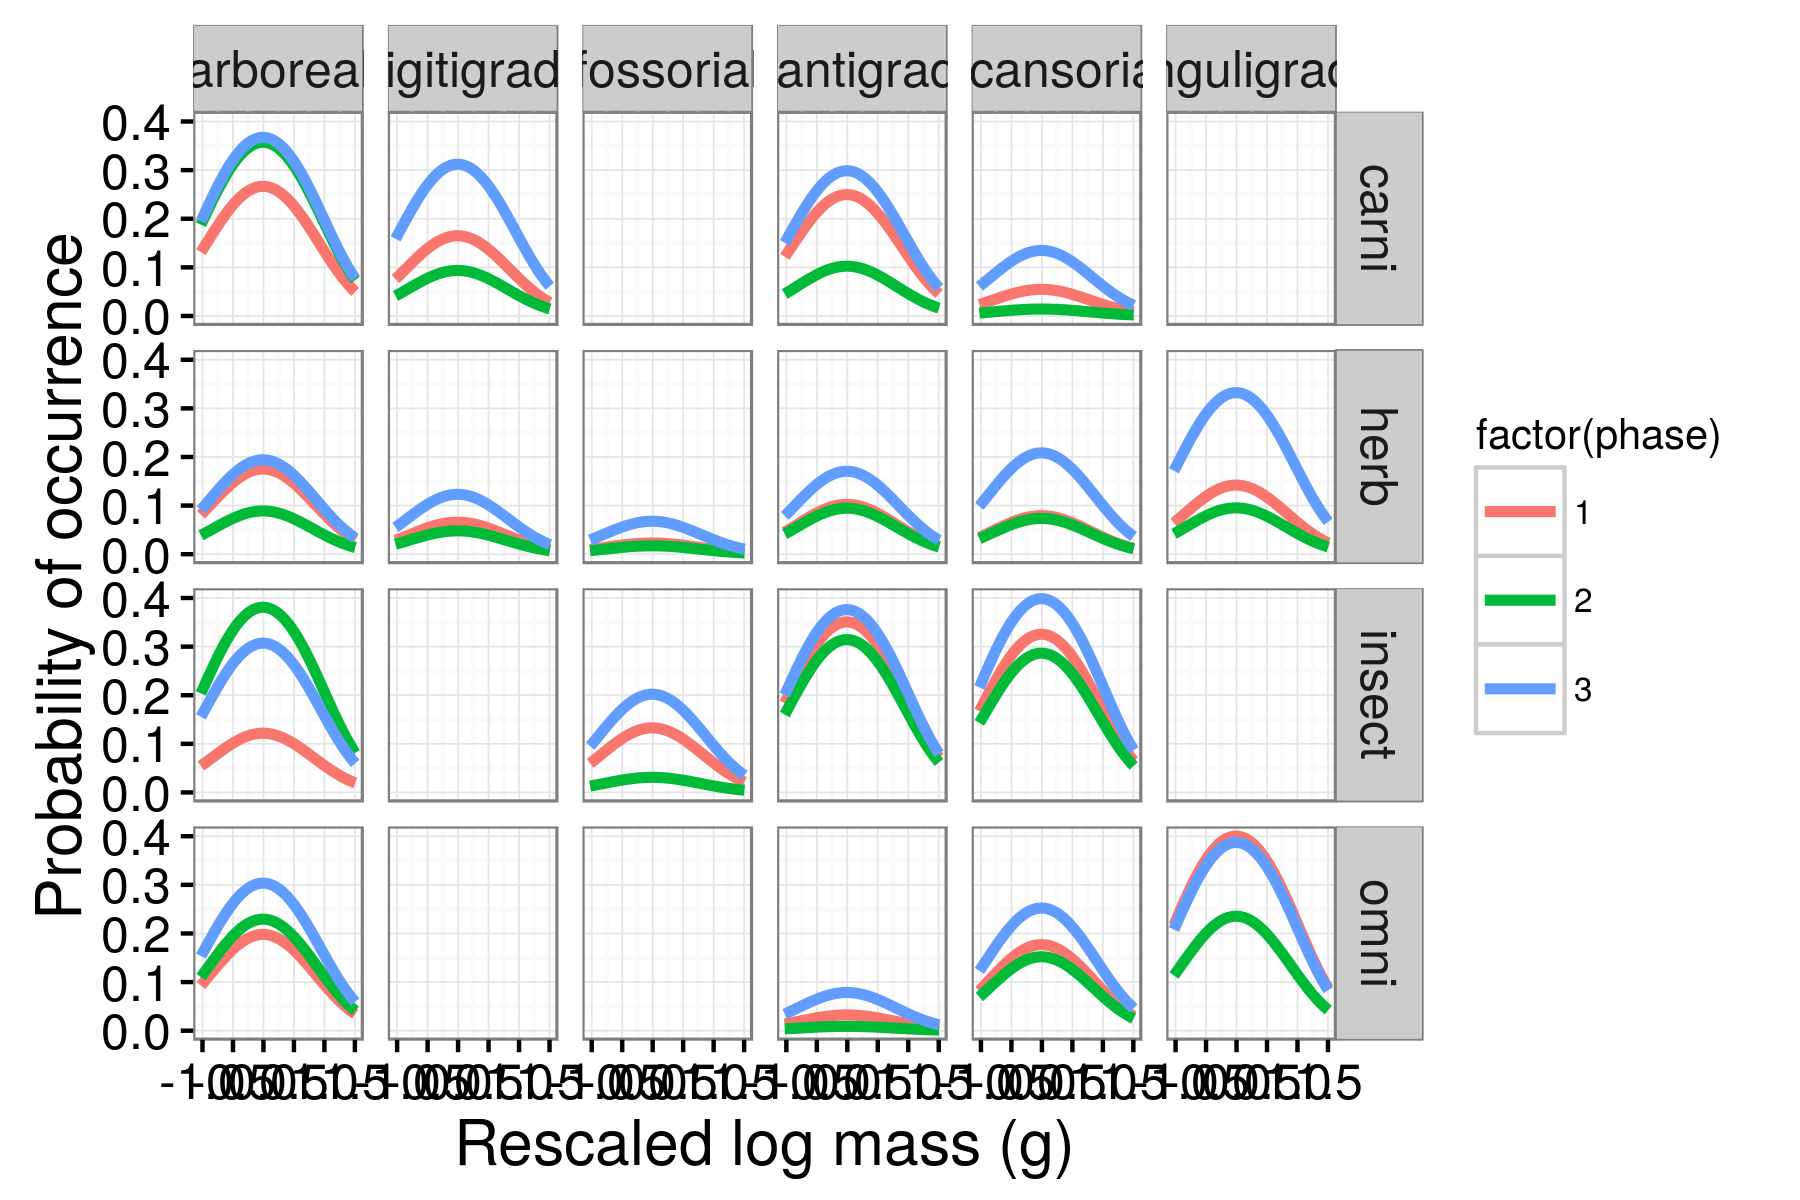
\includegraphics[width=\textwidth,height=0.8\textheight,keepaspectratio=true]{figure/mass_on_pres}
  \caption[Effect of mass on probability of species occurrence as estimated from the pure-presence model]{Mean estimate of the effect of species mass on the probability of a species occurrence for each of the three plant phases. The effect of mass is considered constant over time and that the only aspect of the model that changes with plant phase is the intercept of the relationship between mass and occurrence. The three plant phases are indicated by the color of the line. Mass has been log-transformed, centered, and rescaled; this means that a mass of 0 corresponds to the mean of log-mass of all observed species and that mass is in standard deviation units.}
  \label{fig:mass_occur}
\end{figure}

\begin{figure}[ht]
  \centering
  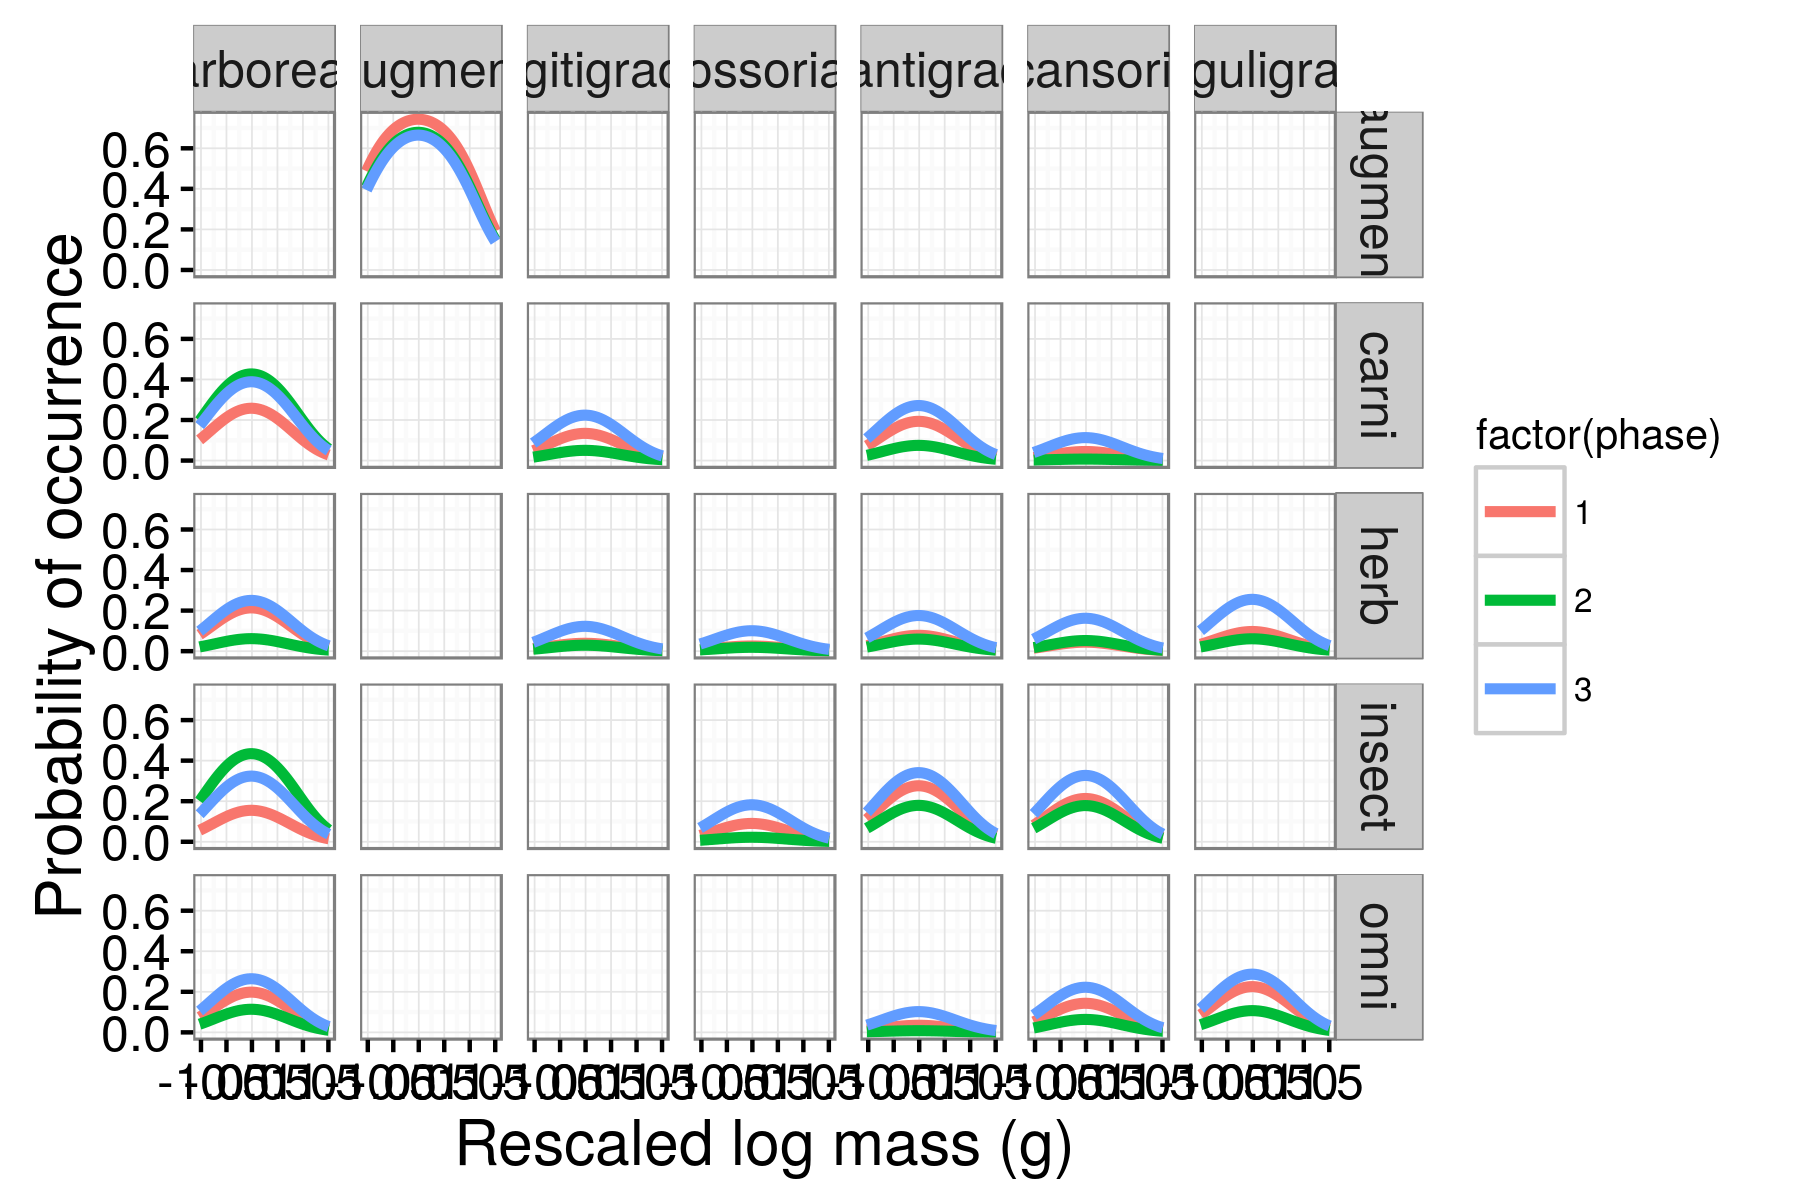
\includegraphics[width=\textwidth,height=0.8\textheight,keepaspectratio=true]{figure/mass_on_origin_bd}
  \caption[Effect of mass on probability of species origination as estimated from the birth-death model]{Mean estimate of the effect of species mass on the probability of a species originating for each of the three plant phases. The effect of mass is considered constant over time and that the only aspect of the model that changes with plant phase is the intercept of the relationship between mass and origination. The three plant phases are indicated by the color of the line. Mass has been log-transformed, centered, and rescaled; this means that a mass of 0 corresponds to the mean of log-mass of all observed species and that mass is in standard deviation units.}
  \label{fig:mass_origin}
\end{figure}

\begin{figure}[ht]
  \centering
  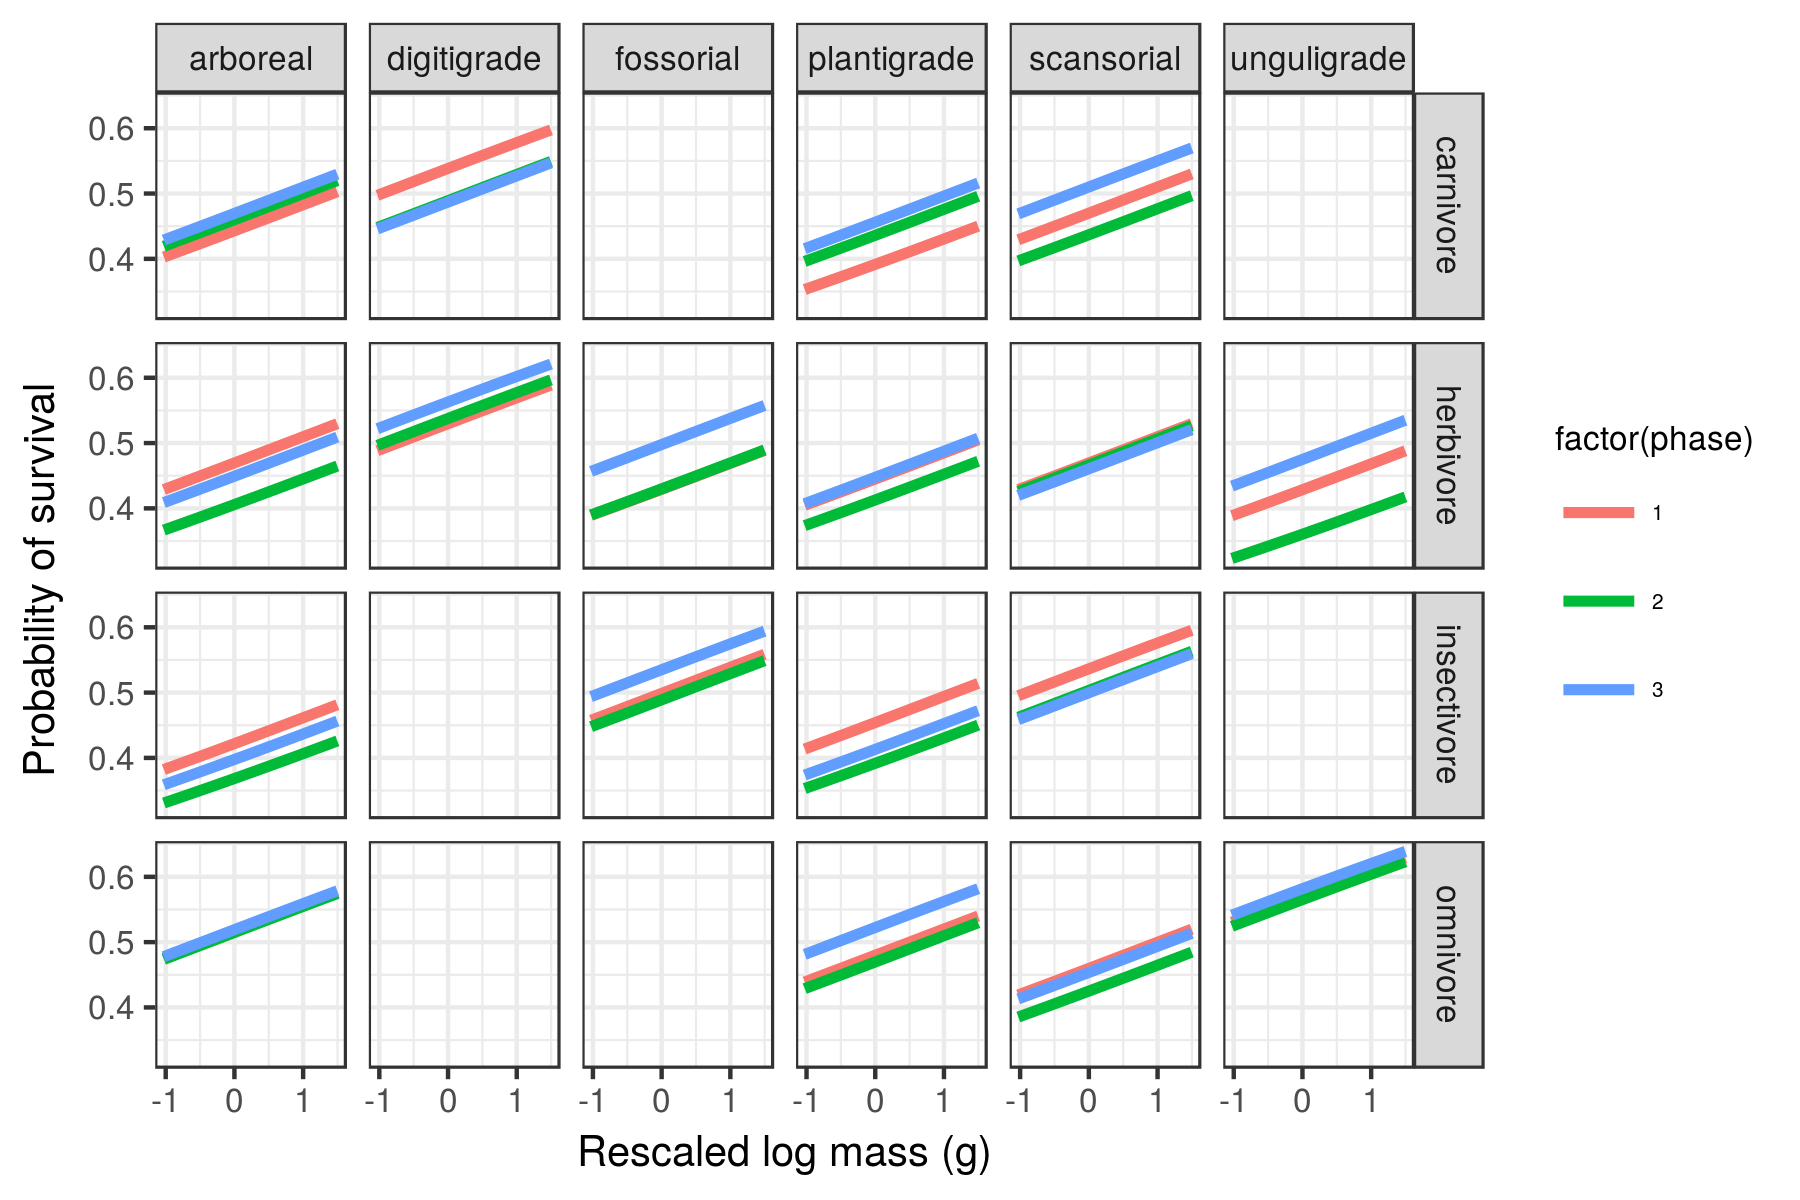
\includegraphics[width=\textwidth,height=0.8\textheight,keepaspectratio=true]{figure/mass_on_surv_bd}
  \caption[Effect of mass on probability of species survival as estimated from the birth-death model]{Mean estimate of the effect of species mass on the probability of a species survival for each of the three plant phases. The effect of mass is considered constant over time and that the only aspect of the model that changes with plant phase is the intercept of the relationship between mass and survival. The three plant phases are indicated by the color of the line. Mass has been log-transformed, centered, and rescaled; this means that a mass of 0 corresponds to the mean of log-mass of all observed species and that mass is in standard deviation units.}
  \label{fig:mass_survival}
\end{figure}

\begin{figure}[ht]
  \centering
  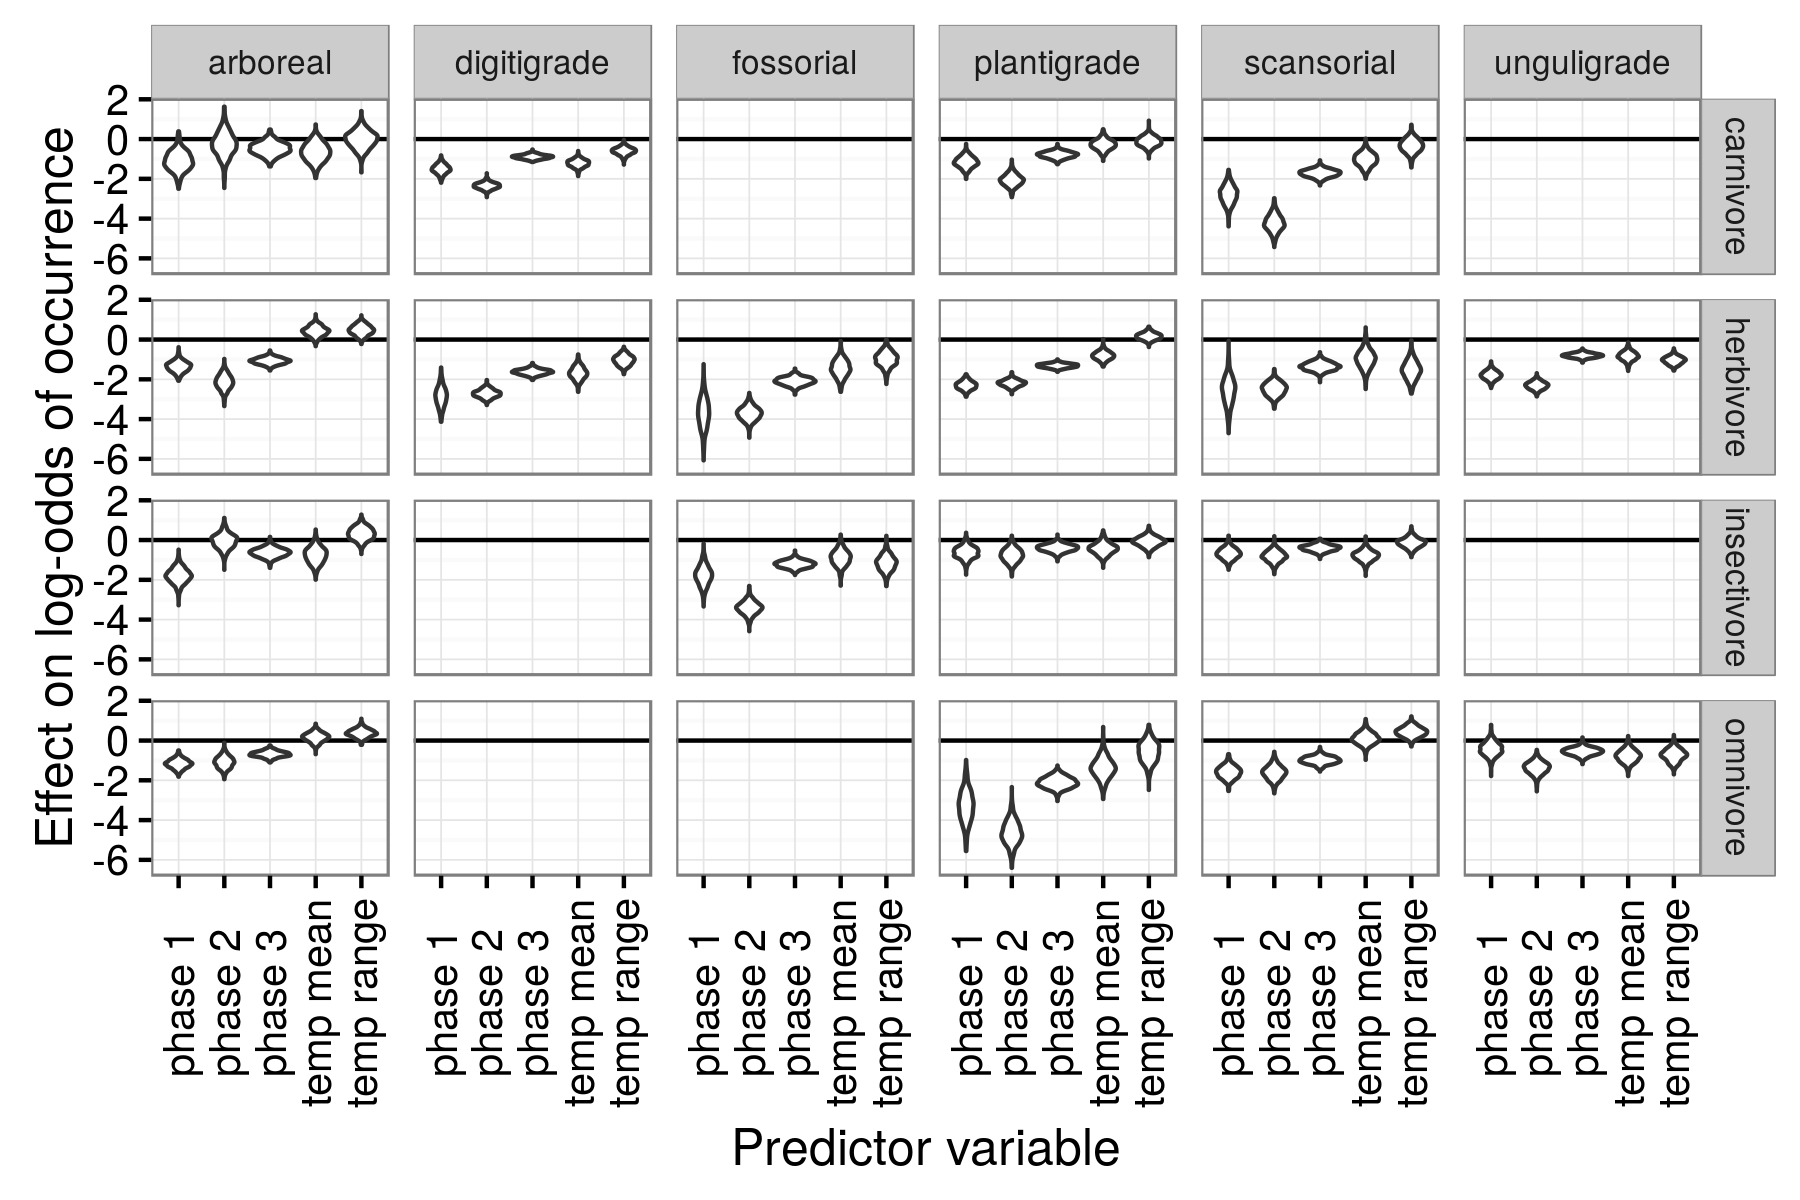
\includegraphics[width=\textwidth,height=0.8\textheight,keepaspectratio=true]{figure/group_on_ecotype}
  \caption[Effects of group-level covariates on log-odds of ecotype occurrence as estimated from the the pure-presence model]{Estimated effects of the group-level covariates describing environmental context on log-odds of species occurrence. These estimates are from the pure-presence model.} 
  \label{fig:group_pure_presence}
\end{figure}

\begin{figure}[ht]
  \centering
  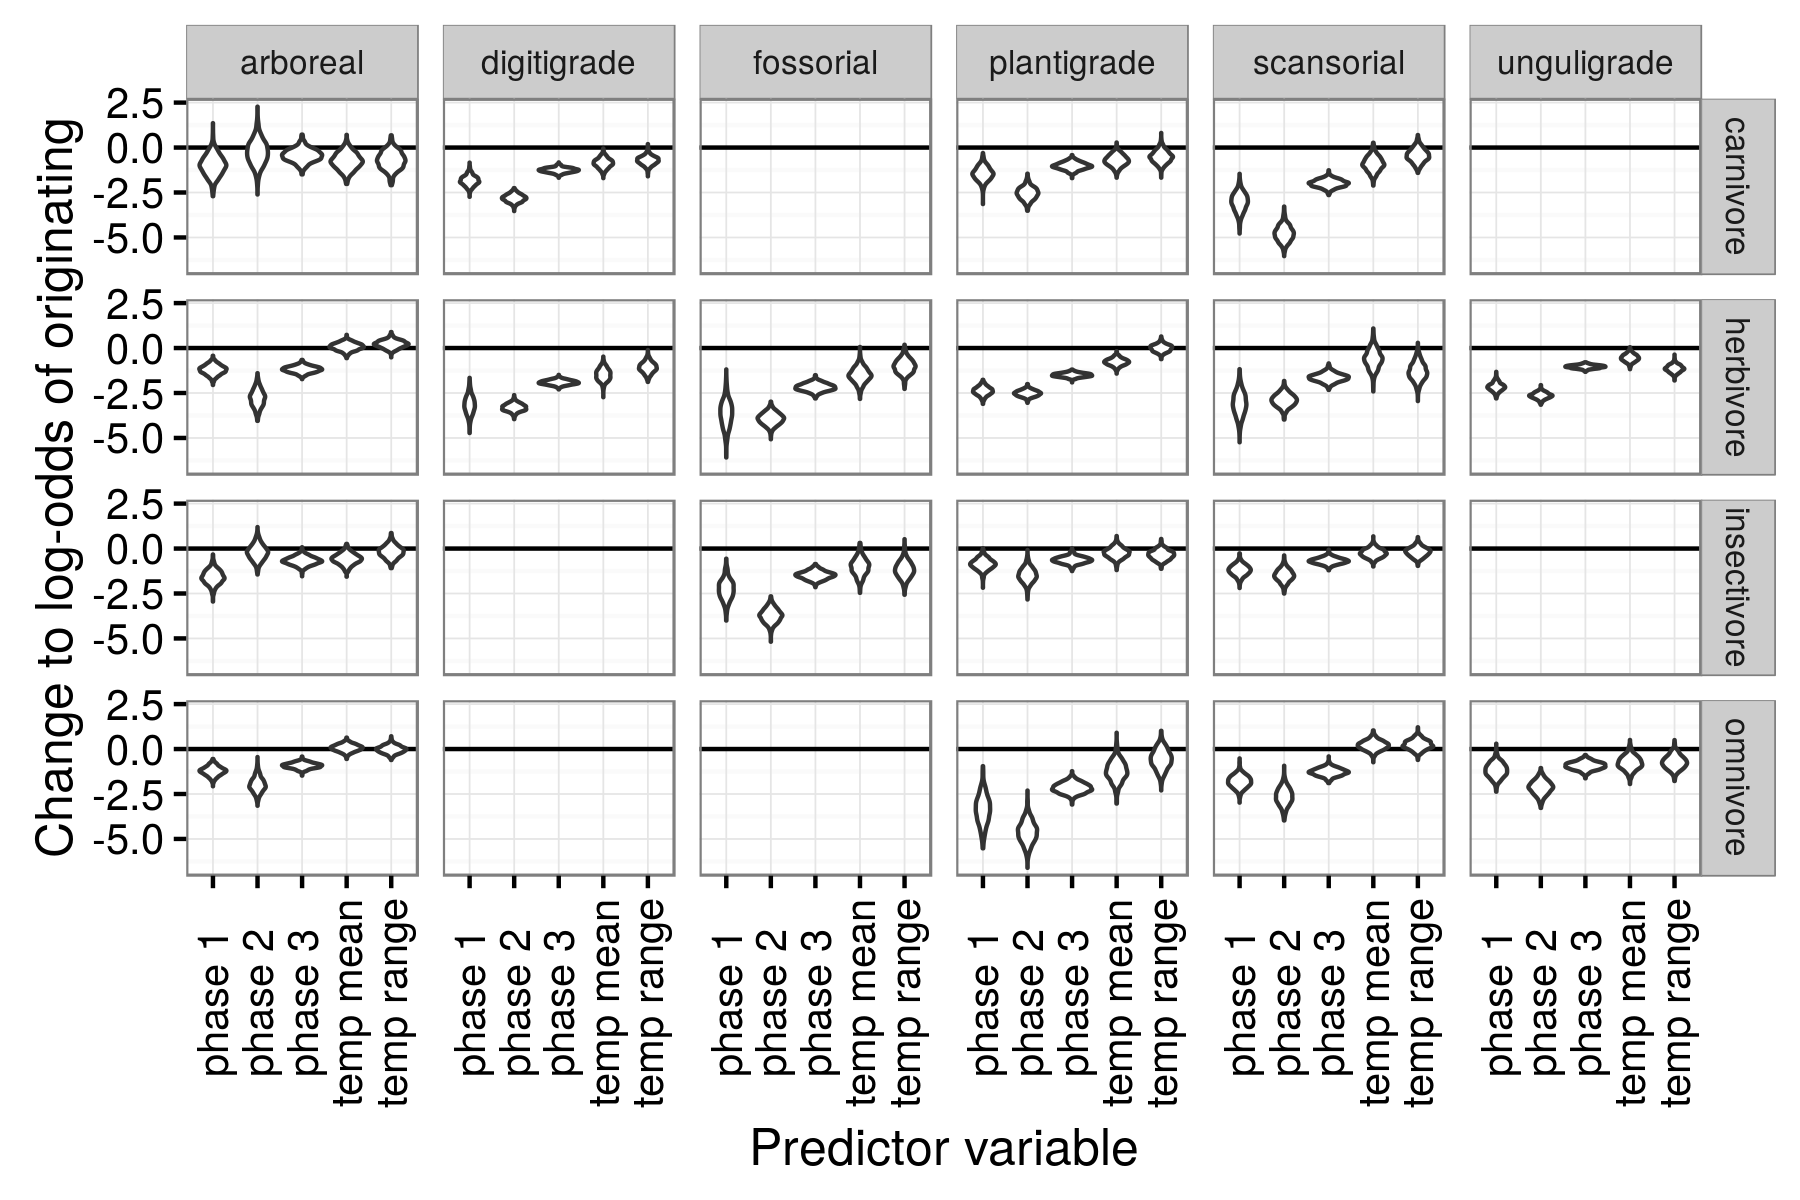
\includegraphics[width=\textwidth,height=0.8\textheight,keepaspectratio=true]{figure/group_on_origin_bd}
  \caption[Effects of group-level covariates on log-odds of ecotype origination as estimated from the the birth-death model]{Estimated effects of the group-level covariates describing environmental context on log-odds of species origination. These estimates are from the birth-death model.}
  \label{fig:group_origin_bd}
\end{figure}

\begin{figure}[ht]
  \centering
  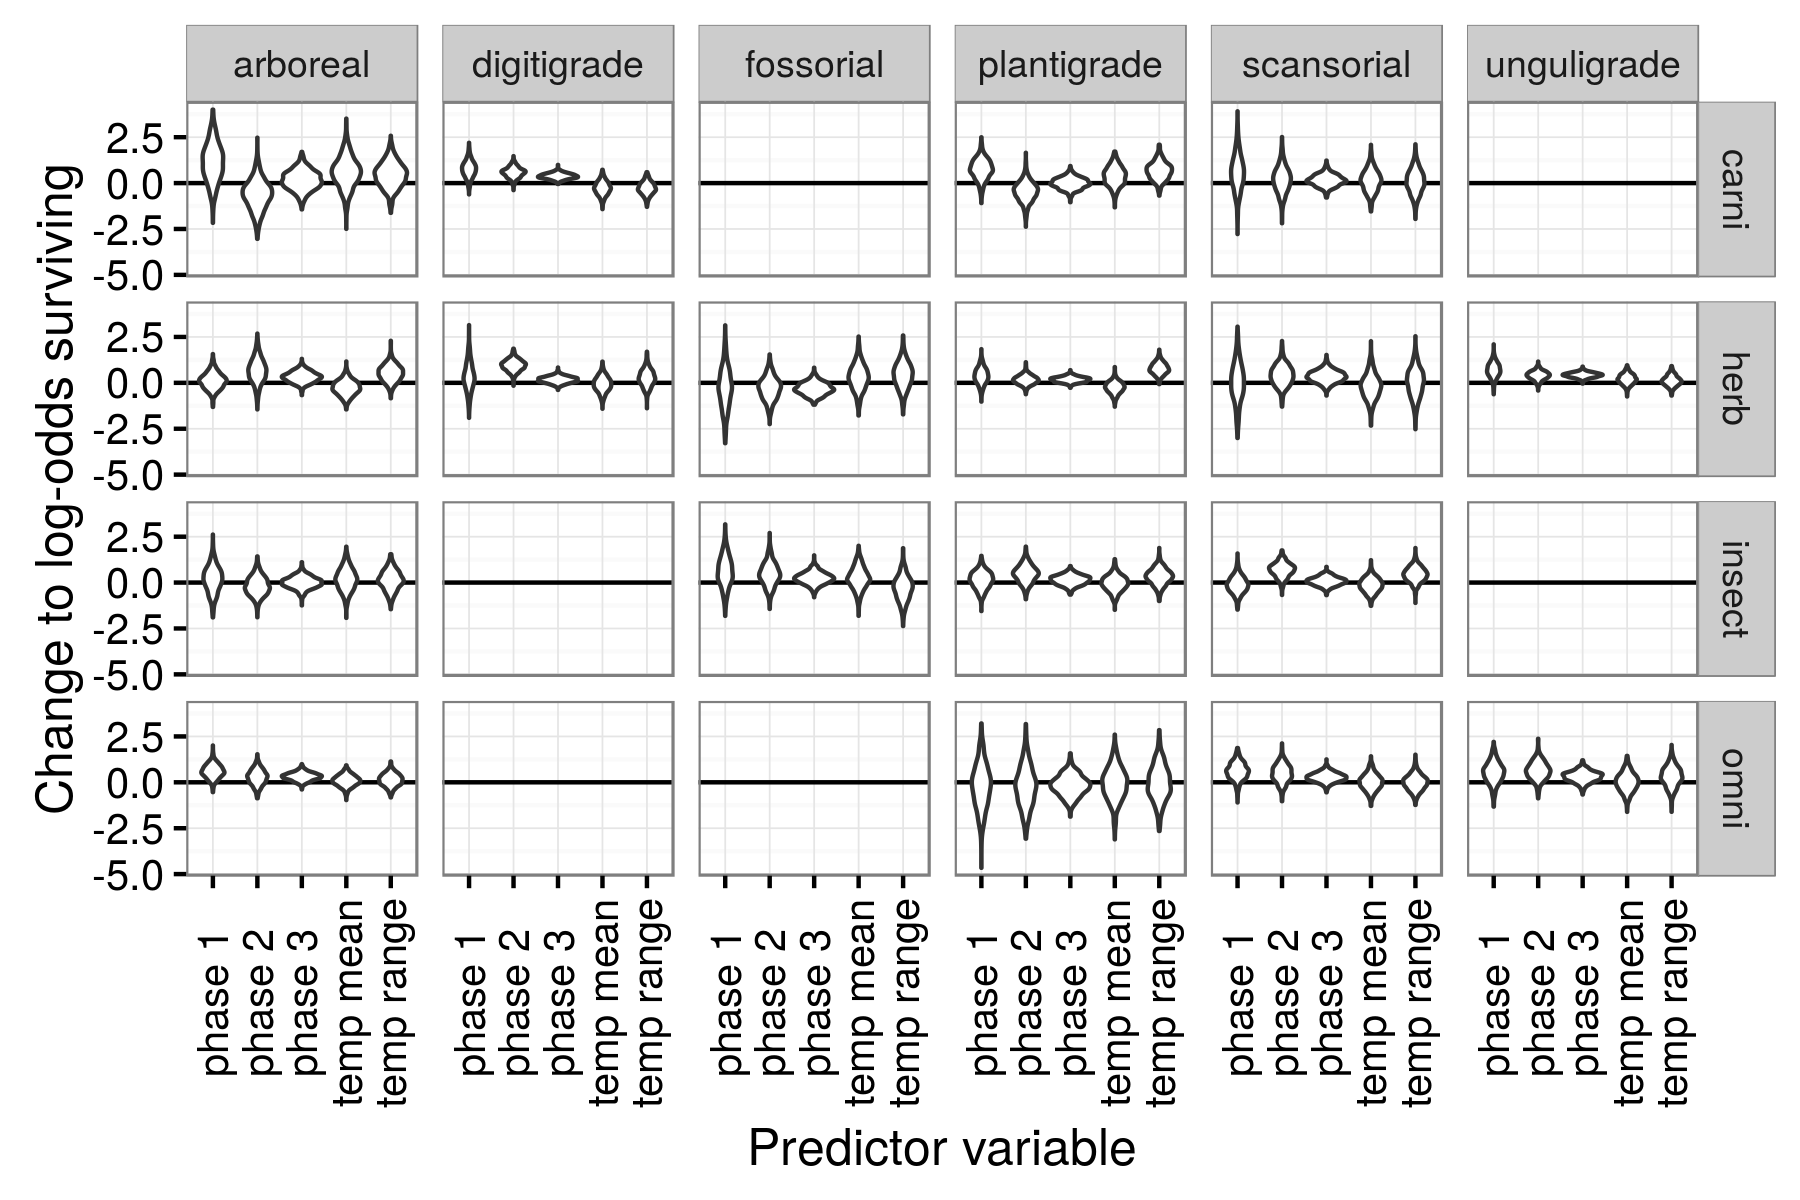
\includegraphics[width=\textwidth,height=0.8\textheight,keepaspectratio=true]{figure/group_on_survival_bd}
  \caption[Effects of group-level covariates on log-odds of ecotype survival as estimated from the the birth-death model]{Estimated effects of the group-level covariates describing environmental context on log-odds of species survlval. These estimates are from the birth-death model.}
  \label{fig:group_surv_bd}
\end{figure}


\subsection*{Analysis of diversity}
\begin{figure}[ht]
  \centering
  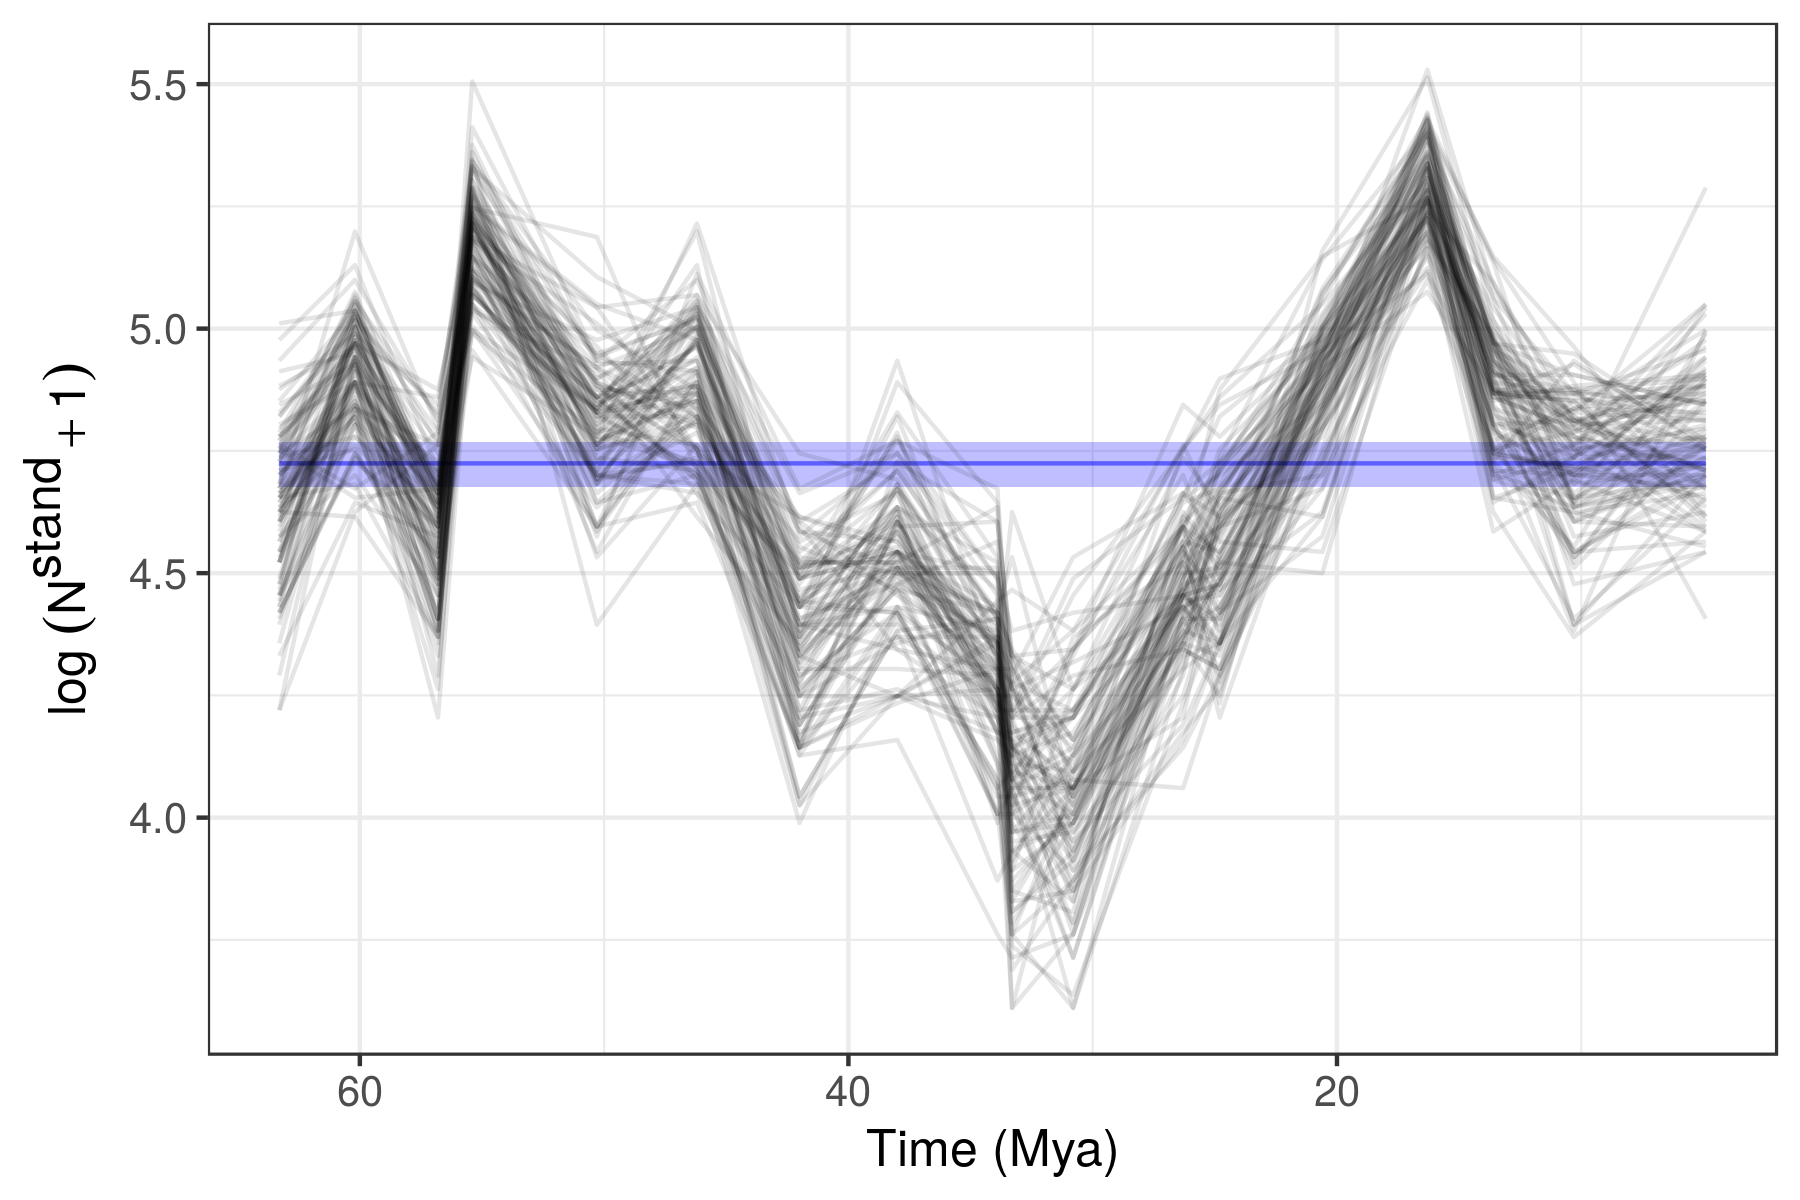
\includegraphics[width=\textwidth,height=0.8\textheight,keepaspectratio=true]{figure/log_diversity}
  \caption[Estimated mammal log-diversity for the Cenozoic]{Posterior of standing log-diversity of North American mammals for the Cenozoic as estimated from the birth-death model; 100 posterior drawsare plotted to indicate the uncertainty in these estimates. The dramatic differences between diversity estimates at the first and second time points and the penultimate and last time points in this series are caused by well known edge effects in discrete-time birth-death models caused by \(p_{\_, t = 1}\) and \(p_{\_, t = T}\) being partially undefiable \citep{Royle2008}; the hierarchical modeling strategy used here helps mitigate these effects but they are still present \citep{Gelman2013d,Royle2008}.}
  \label{fig:diversity_est}
\end{figure}

\begin{figure}[ht]
  \centering
  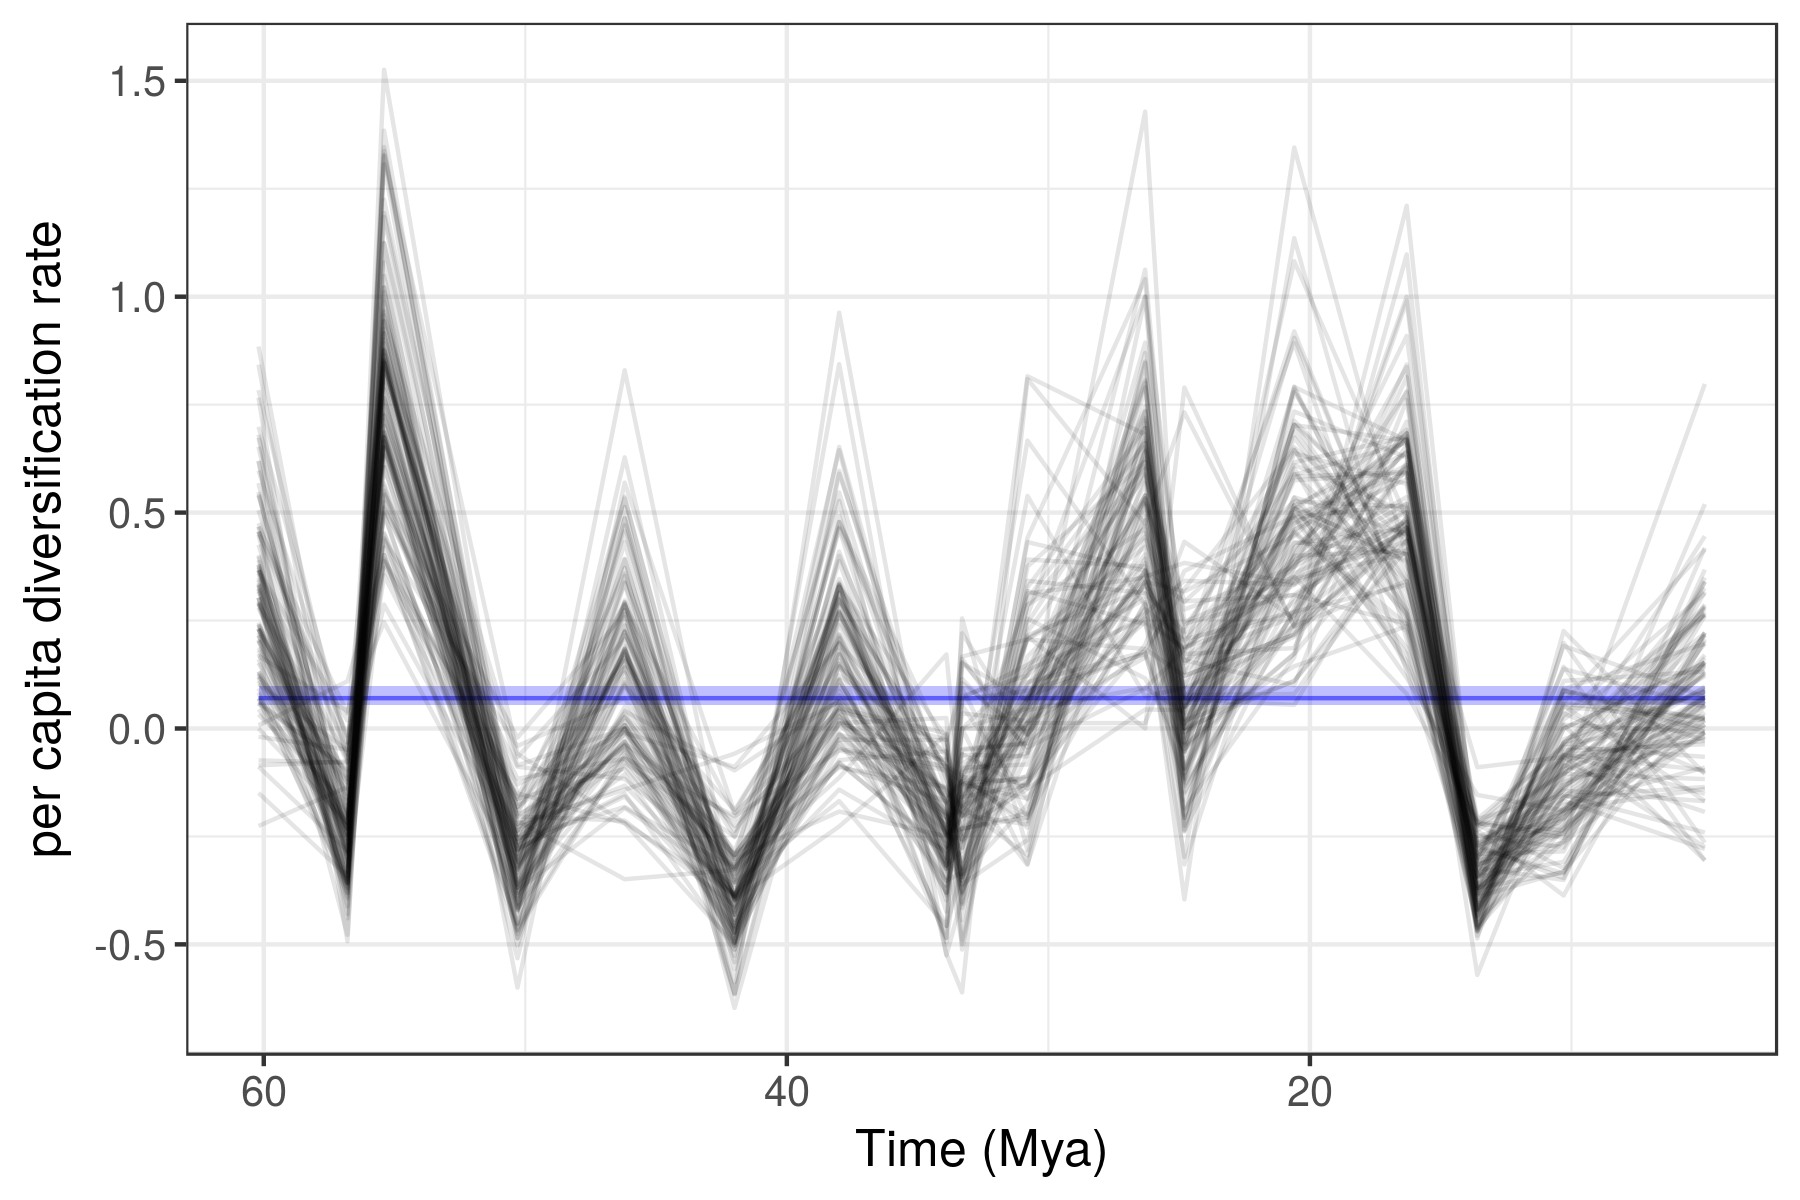
\includegraphics[width=\textwidth,height=0.8\textheight,keepaspectratio=true]{figure/div_rate}
  \caption[Mammal diversification rate estimtes]{Posterior estimates of North American mammal diversification rates for the Cenozoic; 100 estimates are ploted to indicate the uncertainty in these estimates. As a reminder, diversification rate is the difference between origination and extinction rates and is in units of species gained per species present per time unit (2 My).}
  \label{fig:diversity_rate}
\end{figure}

\begin{figure}[ht]
  \centering
  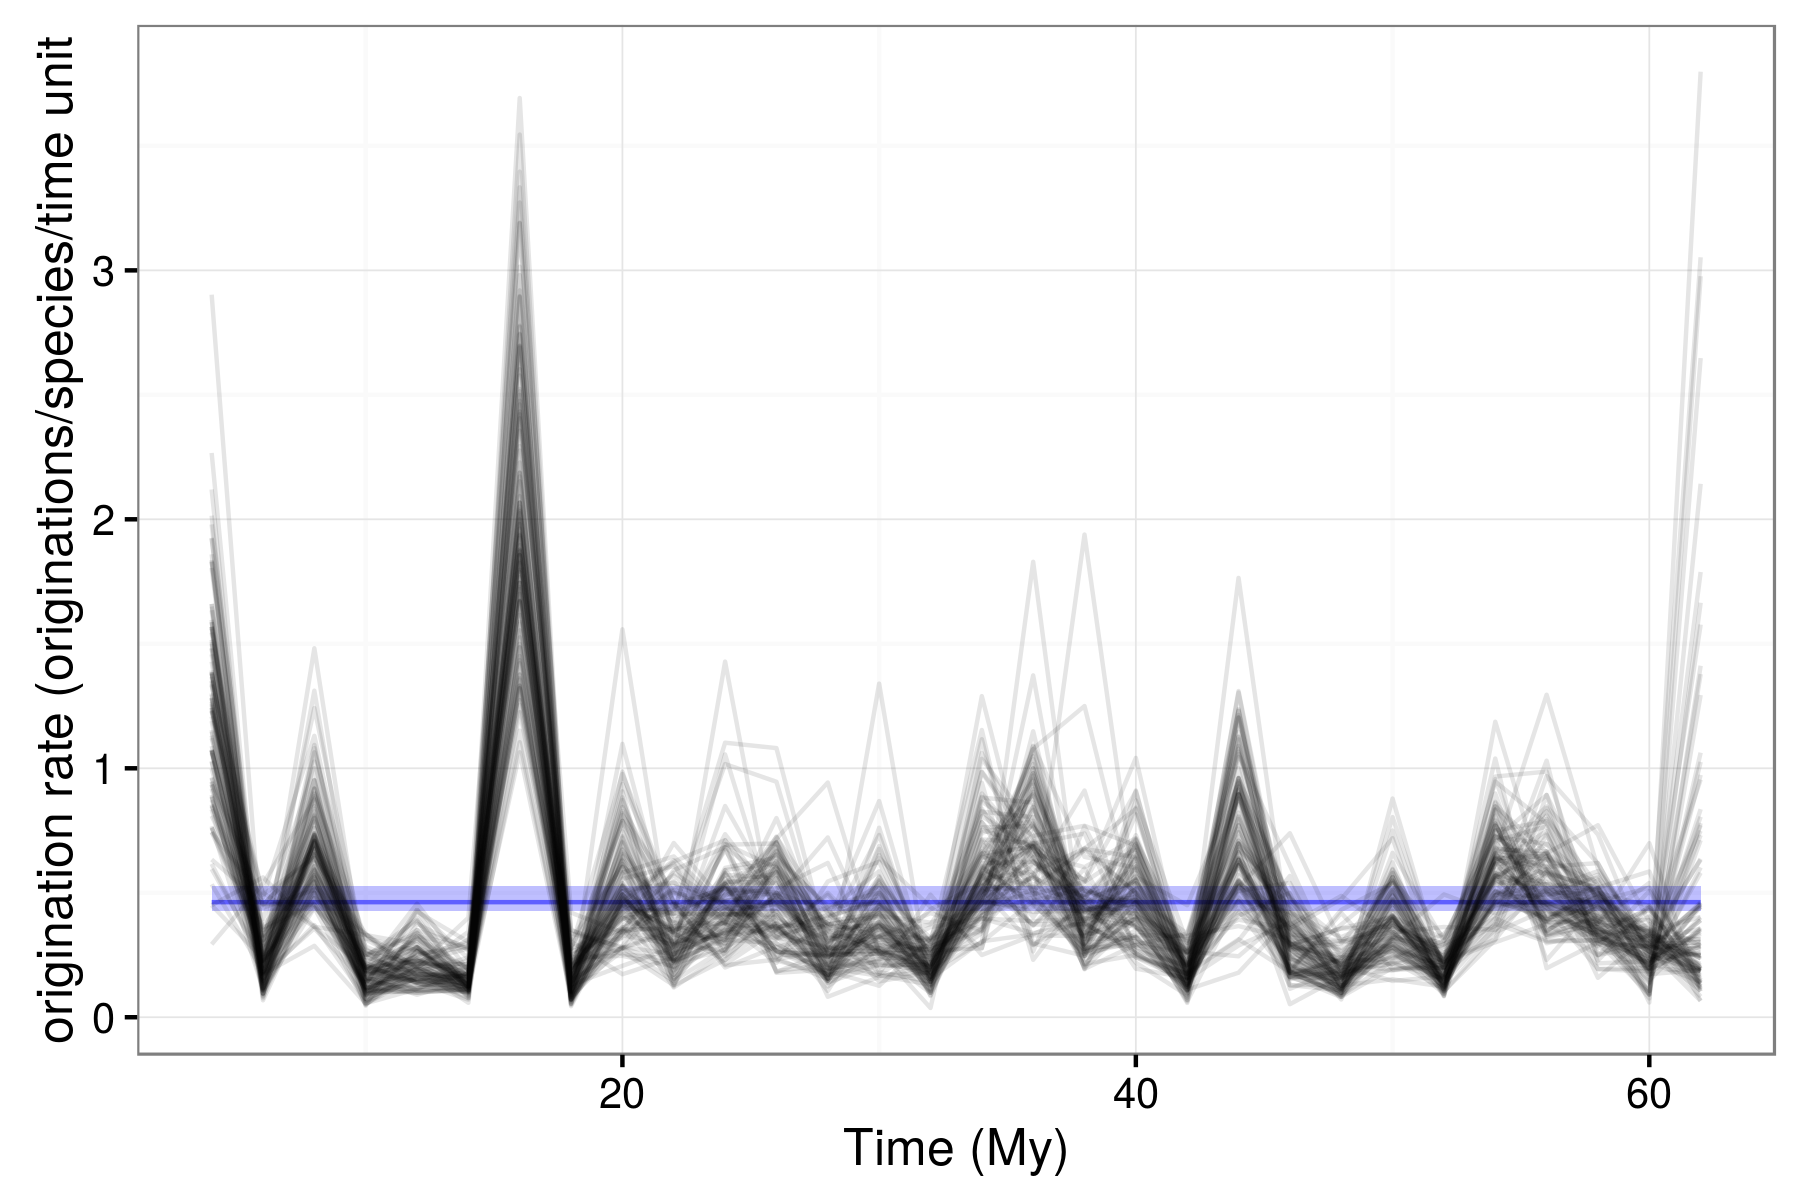
\includegraphics[width=\textwidth,height=0.8\textheight,keepaspectratio=true]{figure/orig_rate}
  \caption{<+caption text+>}
  \label{fig:origin_rate}
\end{figure}

\begin{figure}[ht]
  \centering
  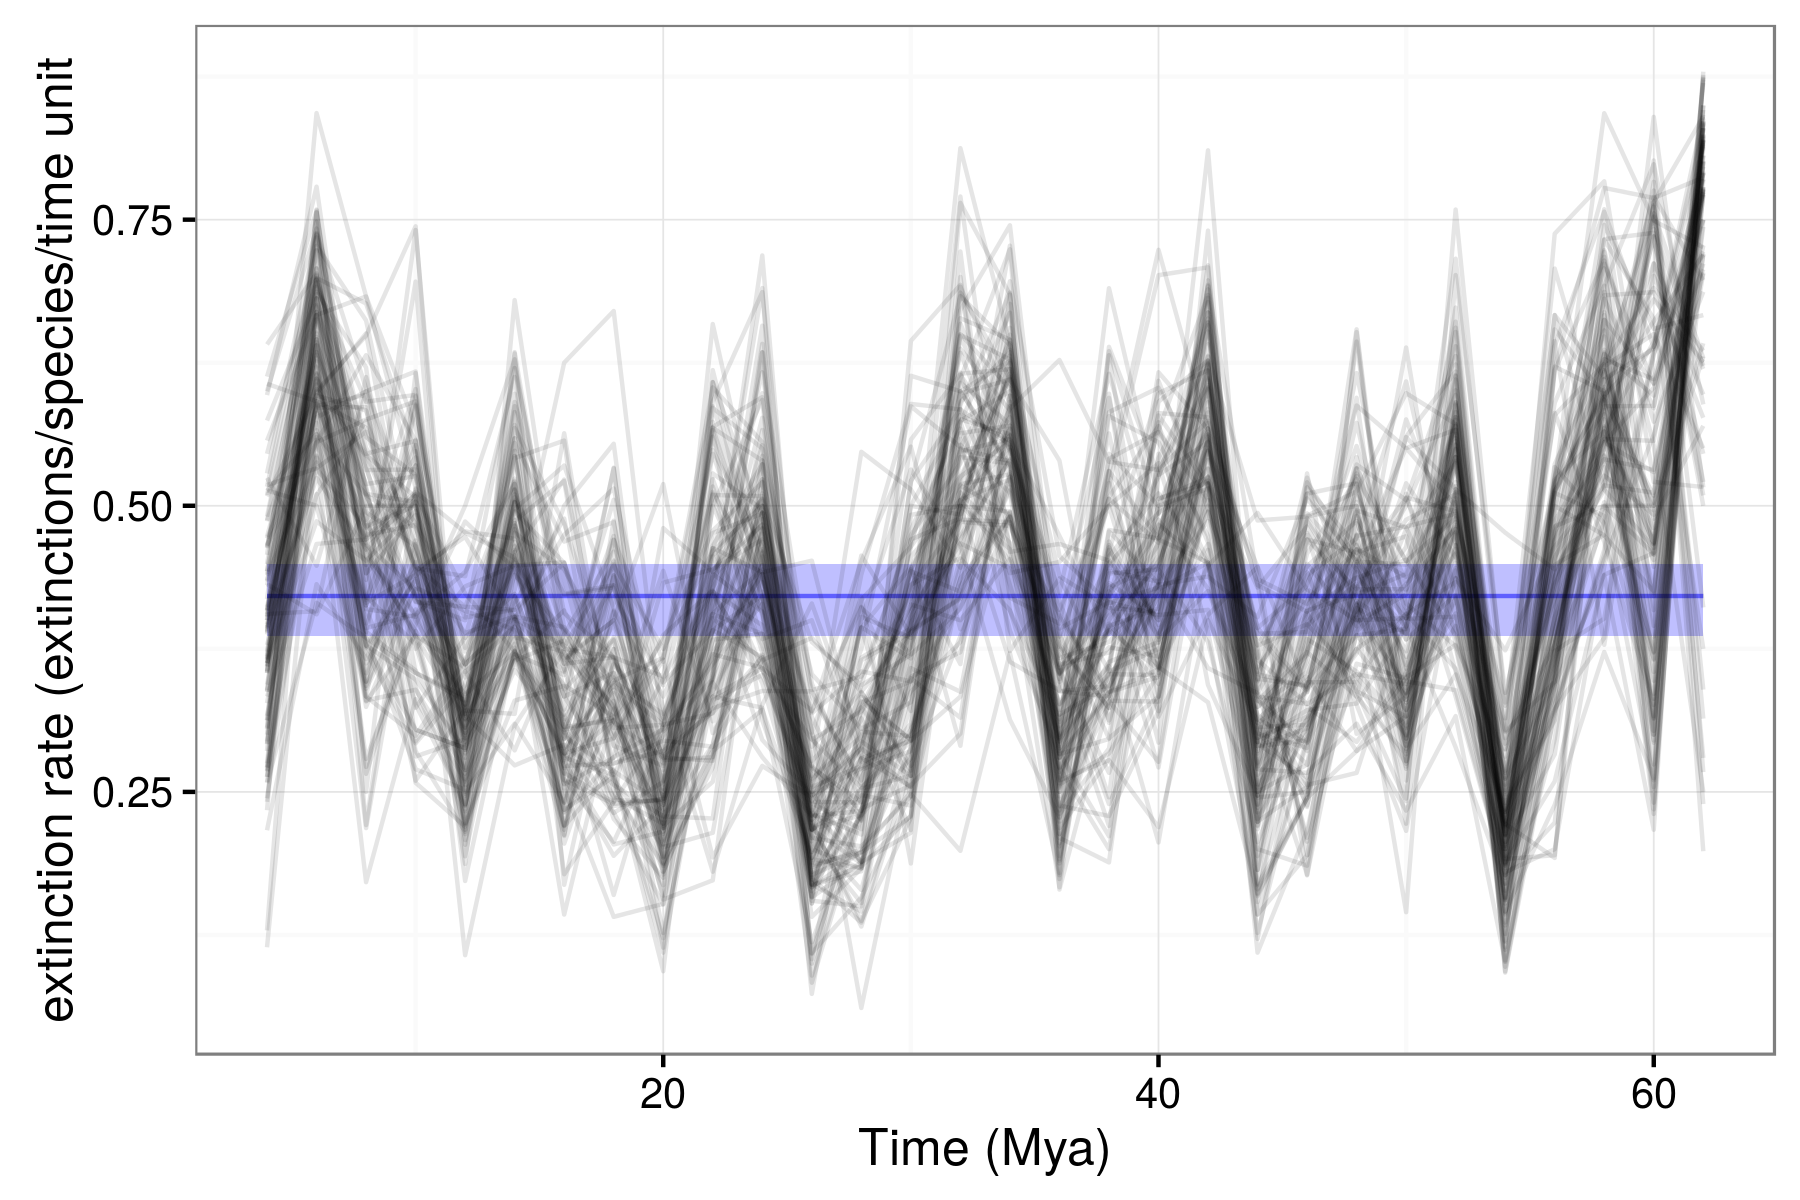
\includegraphics[width=\textwidth,height=0.8\textheight,keepaspectratio=true]{figure/death_rate}
  \caption{<+caption text+>}
  \label{fig:extinct_rate}
\end{figure}


\end{document}
